\documentclass[12pt]{article}
\usepackage{amsmath}
\usepackage{titlesec}
\usepackage{cite}
\usepackage{graphicx}
\usepackage{float}
\usepackage{caption}
\usepackage{subcaption}
\usepackage{wrapfig}
\usepackage{todonotes}
\RequirePackage{filecontents} 
\usepackage[margin=0.5in]{geometry}
\usepackage{cleveref}
\date{}
\titleformat{\subsection}
  {\normalfont\fontsize{11}{17}\sffamily\bfseries\slshape}
  {\thesubsection}
  {1em}
  {}
  
\begin{filecontents*}{\jobname.bib}
@article{dockingrev,
  doi = {10.1016/s1367-5931(02)00339-3},
  url = {http://dx.doi.org/10.1016/S1367-5931(02)00339-3},
  year  = {2002},
  month = {aug},
  publisher = {Elsevier {BV}},
  volume = {6},
  number = {4},
  pages = {439--446},
  author = {Brian K Shoichet and Susan L McGovern and Binqing Wei and John J Irwin},
  title = {Lead discovery using molecular docking},
  journal = {Current Opinion in Chemical Biology}
}
@article{itcref,
  doi = {10.1016/s0959-440x(00)00248-7},
  url = {http://dx.doi.org/10.1016/S0959-440X(00)00248-7},
  year  = {2001},
  month = {sep},
  publisher = {Elsevier {BV}},
  volume = {11},
  number = {5},
  pages = {560--566},
  author = {Stephanie Leavitt and Ernesto Freire},
  title = {Direct measurement of protein binding energetics by isothermal titration calorimetry},
  journal = {Current Opinion in Structural Biology}
}
@article{blast,
  doi = {10.1016/s0022-2836(05)80360-2},
  url = {http://dx.doi.org/10.1016/S0022-2836(05)80360-2},
  year  = {1990},
  month = {oct},
  publisher = {Elsevier {BV}},
  volume = {215},
  number = {3},
  pages = {403--410},
  author = {Stephen F. Altschul and Warren Gish and Webb Miller and Eugene W. Myers and David J. Lipman},
  title = {Basic local alignment search tool},
  journal = {Journal of Molecular Biology}
}
@article{modeller,
  doi = {10.1006/jmbi.1993.1626},
  url = {http://dx.doi.org/10.1006/jmbi.1993.1626},
  year  = {1993},
  month = {dec},
  publisher = {Elsevier {BV}},
  volume = {234},
  number = {3},
  pages = {779--815},
  author = {Andrej {\v{S}}ali and Tom L. Blundell},
  title = {Comparative Protein Modelling by Satisfaction of Spatial Restraints},
  journal = {Journal of Molecular Biology}
}
@article{openmm,
  doi = {10.1021/ct300857j},
  url = {http://dx.doi.org/10.1021/ct300857j},
  year  = {2013},
  month = {jan},
  publisher = {American Chemical Society ({ACS})},
  volume = {9},
  number = {1},
  pages = {461--469},
  author = {Peter Eastman and Mark S. Friedrichs and John D. Chodera and Randall J. Radmer and Christopher M. Bruns and Joy P. Ku and Kyle A. Beauchamp and Thomas J. Lane and Lee-Ping Wang and Diwakar Shukla and Tony Tye and Mike Houston and Timo Stich and Christoph Klein and Michael R. Shirts and Vijay S. Pande},
  title = {{OpenMM} 4: A Reusable,  Extensible,  Hardware Independent Library for High Performance Molecular Simulation},
  journal = {J. Chem. Theory Comput.}
}
@article{shirts2008,
  doi = {10.1063/1.2978177},
  url = {http://dx.doi.org/10.1063/1.2978177},
  year  = {2008},
  publisher = {{AIP} Publishing},
  volume = {129},
  number = {12},
  pages = {124105},
  author = {Michael R. Shirts and John D. Chodera},
  title = {Statistically optimal analysis of samples from multiple equilibrium states},
  journal = {J. Chem. Phys.}
}
@book{liu,
  author = "Jun S. Liu",
  title = "Monte Carlo strategies in scientific computing",
  publisher = "Springer",
  year = "2001",
  ISBN = "0387952306"
}
@article{kyle,
  doi = {10.1021/ct200463m},
  url = {http://dx.doi.org/10.1021/ct200463m},
  year  = {2011},
  month = {oct},
  publisher = {American Chemical Society ({ACS})},
  volume = {7},
  number = {10},
  pages = {3412--3419},
  author = {Kyle A. Beauchamp and Gregory R. Bowman and Thomas J. Lane and Lutz Maibaum and Imran S. Haque and Vijay S. Pande},
  title = {{MSMBuilder}2: Modeling Conformational Dynamics on the Picosecond to Millisecond Scale},
  journal = {J. Chem. Theory Comput.}
}
@Article{rasgtp,
   Author="Pai, E. F.  and Krengel, U.  and Petsko, G. A.  and Goody, R. S.  and Kabsch, W.  and Wittinghofer, A. ",
   Title="{{R}efined crystal structure of the triphosphate conformation of {H}-ras p21 at 1.35 {A} resolution: implications for the mechanism of {G}{T}{P} hydrolysis}",
   Journal="EMBO J.",
   Year="1990",
   Volume="9",
   Number="8",
   Pages="2351--2359",
   Month="Aug"
}
@article{rasgdp,
  doi = {10.1016/0022-2836(91)90753-s},
  url = {http://dx.doi.org/10.1016/0022-2836(91)90753-S},
  year  = {1991},
  month = {feb},
  publisher = {Elsevier {BV}},
  volume = {217},
  number = {3},
  pages = {503--516},
  author = {Liang Tong and Abraham M. de Vos and Michael V. Milburn and Sung-Hou Kim},
  title = {Crystal structures at 2.2 {\{AA}} resolution of the catalytic domains of normal ras protein and an oncogenic mutant complexed with {GDP}},
  journal = {Journal of Molecular Biology}
}
@article{deshaw,
  doi = {10.1371/journal.pone.0032131},
  url = {http://dx.doi.org/10.1371/journal.pone.0032131},
  year  = {2012},
  month = {feb},
  publisher = {Public Library of Science ({PLoS})},
  volume = {7},
  number = {2},
  pages = {e32131},
  author = {Kresten Lindorff-Larsen and Paul Maragakis and Stefano Piana and Michael P. Eastwood and Ron O. Dror and David E. Shaw},
  editor = {Daniel J. Muller},
  title = {Systematic Validation of Protein Force Fields against Experimental Data},
  journal = {{PLoS} {ONE}}
}
@article{craik,
  doi = {10.1126/science.1169378},
  url = {http://dx.doi.org/10.1126/science.1169378},
  year  = {2009},
  month = {apr},
  publisher = {American Association for the Advancement of Science ({AAAS})},
  volume = {324},
  number = {5924},
  pages = {213--215},
  author = {G. M. Lee and C. S. Craik},
  title = {Trapping Moving Targets with Small Molecules},
  journal = {Science}
}
@article{mark,
  doi = {10.1016/s1093-3263(00)80091-1},
  url = {http://dx.doi.org/10.1016/S1093-3263(00)80091-1},
  year  = {2000},
  month = {jan},
  publisher = {Elsevier {BV}},
  volume = {18},
  number = {4-5},
  pages = {452--463},
  author = {John M. Barnard and Geoff M. Downs and Annette von Scholley-Pfab and Robert D. Brown},
  title = {Use of Markush structure analysis techniques for descriptor generation and clustering of large combinatorial libraries},
  journal = {Journal of Molecular Graphics and Modelling}
}
@article{pyla,
  doi = {10.1038/nrc3106},
  url = {http://dx.doi.org/10.1038/nrc3106},
  year  = {2011},
  month = {oct},
  publisher = {Nature Publishing Group},
  volume = {11},
  number = {11},
  pages = {761--774},
  author = {Yuliya Pylayeva-Gupta and Elda Grabocka and Dafna Bar-Sagi},
  title = {{RAS} oncogenes: weaving a tumorigenic web},
  journal = {Nat Rev Cancer}
}
@article{kitchen2004,
  doi = {10.1038/nrd1549},
  url = {http://dx.doi.org/10.1038/nrd1549},
  year  = {2004},
  month = {nov},
  publisher = {Nature Publishing Group},
  volume = {3},
  number = {11},
  pages = {935--949},
  author = {Douglas B. Kitchen and H{\'{e}}l{\`{e}}ne Decornez and John R. Furr and J\"{u}rgen Bajorath},
  title = {Docking and scoring in virtual screening for drug discovery: methods and applications},
  journal = {Nat Rev Drug Discov}
}
@article{lyubartsev1992,
  doi = {10.1063/1.462133},
  url = {http://dx.doi.org/10.1063/1.462133},
  year  = {1992},
  publisher = {{AIP} Publishing},
  volume = {96},
  number = {3},
  pages = {1776},
  author = {A. P. Lyubartsev and A. A. Martsinovski and S. V. Shevkunov and P. N. Vorontsov-Velyaminov},
  title = {New approach to Monte Carlo calculation of the free energy: Method of expanded ensembles},
  journal = {J. Chem. Phys.}
}
@article{warren2006,
  doi = {10.1021/jm050362n},
  url = {http://dx.doi.org/10.1021/jm050362n},
  year  = {2006},
  month = {oct},
  publisher = {American Chemical Society ({ACS})},
  volume = {49},
  number = {20},
  pages = {5912--5931},
  author = {Gregory L. Warren and C. Webster Andrews and Anna-Maria Capelli and Brian Clarke and Judith LaLonde and Millard H. Lambert and Mika Lindvall and Neysa Nevins and Simon F. Semus and Stefan Senger and Giovanna Tedesco and Ian D. Wall and James M. Woolven and Catherine E. Peishoff and Martha S. Head},
  title = {A Critical Assessment of Docking Programs and Scoring Functions},
  journal = {Journal of Medicinal Chemistry}
}
@article{kuntz1999,
  doi = {10.1073/pnas.96.18.9997},
  url = {http://dx.doi.org/10.1073/pnas.96.18.9997},
  year  = {1999},
  month = {aug},
  publisher = {Proceedings of the National Academy of Sciences},
  volume = {96},
  number = {18},
  pages = {9997--10002},
  author = {I. D. Kuntz and K. Chen and K. A. Sharp and P. A. Kollman},
  title = {The maximal affinity of ligands},
  journal = {Proceedings of the National Academy of Sciences}
}
@article{perez2013,
  doi = {10.1063/1.4811489},
  url = {http://dx.doi.org/10.1063/1.4811489},
  year  = {2013},
  publisher = {{AIP} Publishing},
  volume = {139},
  number = {1},
  pages = {015102},
  author = {Guillermo Perez-Hernandez and Fabian Paul and Toni Giorgino and Gianni De Fabritiis and Frank Noe},
  title = {Identification of slow molecular order parameters for Markov model construction},
  journal = {J. Chem. Phys.}
}
@article{boresch2013,
  doi = {10.1021/jp0217839},
  url = {http://dx.doi.org/10.1021/jp0217839},
  year  = {2003},
  month = {sep},
  publisher = {American Chemical Society ({ACS})},
  volume = {107},
  number = {35},
  pages = {9535--9551},
  author = {Stefan Boresch and Franz Tettinger and Martin Leitgeb and Martin Karplus},
  title = {Absolute Binding Free Energies:~ A Quantitative Approach for Their Calculation},
  journal = {J. Phys. Chem. B}
}
@article{mak2014,
  doi = {10.1016/j.cllc.2014.09.005},
  url = {http://dx.doi.org/10.1016/j.cllc.2014.09.005},
  year  = {2014},
  month = {sep},
  publisher = {Elsevier {BV}},
  author = {Raymond H. Mak and Gretchen Hermann and John H. Lewis and Hugo J.W.L. Aerts and Elizabeth H. Baldini and Aileen B. Chen and Yolonda L. Colson and Fred H. Hacker and David Kozono and Jon O. Wee and Yu-Hui Chen and Paul J. Catalano and Kwok-Kin Wong and David J. Sher},
  title = {Outcomes by Tumor Histology and {KRAS} Mutation Status after Lung Stereotactic Body Radiation Therapy for Early Stage Non-Small Cell Lung Cancer},
  journal = {Clinical Lung Cancer}
}
@article{pi3k,
  doi = {10.1016/s0092-8674(00)00196-3},
  url = {http://dx.doi.org/10.1016/S0092-8674(00)00196-3},
  year  = {2000},
  month = {dec},
  publisher = {Elsevier {BV}},
  volume = {103},
  number = {6},
  pages = {931--944},
  author = {Michael E. Pacold and Sabine Suire and Olga Perisic and Samuel Lara-Gonzalez and Colin T. Davis and Edward H. Walker and Phillip T. Hawkins and Len Stephens and John F. Eccleston and Roger L. Williams},
  title = {Crystal Structure and Functional Analysis of Ras Binding to Its Effector Phosphoinositide 3-Kinase $\upgamma$},
  journal = {Cell}
}
@article{chodera,
  doi = {10.1063/1.3660669},
  url = {http://dx.doi.org/10.1063/1.3660669},
  year  = {2011},
  publisher = {{AIP} Publishing},
  volume = {135},
  number = {19},
  pages = {194110},
  author = {John D. Chodera and Michael R. Shirts},
  title = {Replica exchange and expanded ensemble simulations as Gibbs sampling: Simple improvements for enhanced mixing},
  journal = {J. Chem. Phys.}
}
@article{trpmut,
  doi = {10.1021/bi00098a002},
  url = {http://dx.doi.org/10.1021/bi00098a002},
  year  = {1991},
  month = {aug},
  publisher = {American Chemical Society ({ACS})},
  volume = {30},
  number = {34},
  pages = {8287--8295},
  author = {Bruno Antonny and Pierre Chardin and Michel Roux and Marc Chabre},
  title = {{GTP} hydrolysis mechanisms in ras p21 and in the ras-{GAP} complex studied by fluorescence measurements on tryptophan mutants},
  journal = {Biochemistry}
}
@article{chodera2014,
  doi = {10.1016/j.sbi.2014.04.002},
  url = {http://dx.doi.org/10.1016/j.sbi.2014.04.002},
  year  = {2014},
  month = {apr},
  publisher = {Elsevier {BV}},
  volume = {25},
  pages = {135--144},
  author = {John D Chodera and Frank No{\'{e}}},
  title = {Markov state models of biomolecular conformational dynamics},
  journal = {Current Opinion in Structural Biology}
}
@article{irwin2012,
  doi = {10.1021/ci3001277},
  url = {http://dx.doi.org/10.1021/ci3001277},
  year  = {2012},
  month = {jul},
  publisher = {American Chemical Society ({ACS})},
  volume = {52},
  number = {7},
  pages = {1757--1768},
  author = {John J. Irwin and Teague Sterling and Michael M. Mysinger and Erin S. Bolstad and Ryan G. Coleman},
  title = {{ZINC}: A Free Tool to Discover Chemistry for Biology},
  journal = {Journal of Chemical Information and Modeling}
}
@article{ostrem2013,
  doi = {10.1038/nature12796},
  url = {http://dx.doi.org/10.1038/nature12796},
  year  = {2013},
  month = {nov},
  publisher = {Nature Publishing Group},
  volume = {503},
  number = {7477},
  pages = {548--551},
  author = {Jonathan M. Ostrem and Ulf Peters and Martin L. Sos and James A. Wells and Kevan M. Shokat},
  title = {K-Ras(G12C) inhibitors allosterically control {GTP} affinity and effector interactions},
  journal = {Nature}
}
@article{bowman2012,
  doi = {10.1073/pnas.1209309109},
  url = {http://dx.doi.org/10.1073/pnas.1209309109},
  year  = {2012},
  month = {jul},
  publisher = {Proceedings of the National Academy of Sciences},
  volume = {109},
  number = {29},
  pages = {11681--11686},
  author = {G. R. Bowman and P. L. Geissler},
  title = {Equilibrium fluctuations of a single folded protein reveal a multitude of potential cryptic allosteric sites},
  journal = {Proceedings of the National Academy of Sciences}
}
@article{hendlich1997,
  doi = {10.1016/s1093-3263(98)00002-3},
  url = {http://dx.doi.org/10.1016/S1093-3263(98)00002-3},
  year  = {1997},
  month = {dec},
  publisher = {Elsevier {BV}},
  volume = {15},
  number = {6},
  pages = {359--363},
  author = {Manfred Hendlich and Friedrich Rippmann and Gerhard Barnickel},
  title = {{LIGSITE}: automatic and efficient detection of potential small molecule-binding sites in proteins},
  journal = {Journal of Molecular Graphics and Modelling}
}
@article{sun2012,
  doi = {10.1002/anie.201201358},
  url = {http://dx.doi.org/10.1002/anie.201201358},
  year  = {2012},
  month = {may},
  publisher = {Wiley-Blackwell},
  volume = {51},
  number = {25},
  pages = {6140--6143},
  author = {Qi Sun and Jason P. Burke and Jason Phan and Michael C. Burns and Edward T. Olejniczak and Alex G. Waterson and Taekyu Lee and Olivia W. Rossanese and Stephen W. Fesik},
  title = {Discovery of Small Molecules that Bind to K-Ras and Inhibit Sos-Mediated Activation},
  journal = {Angew. Chem. Int. Ed.}
}
@article{gilson1997,
  doi = {10.1016/s0006-3495(97)78756-3},
  url = {http://dx.doi.org/10.1016/S0006-3495(97)78756-3},
  year  = {1997},
  month = {mar},
  publisher = {Elsevier {BV}},
  volume = {72},
  number = {3},
  pages = {1047--1069},
  author = {M.K. Gilson and J.A. Given and B.L. Bush and J.A. McCammon},
  title = {The statistical-thermodynamic basis for computation of binding affinities: a critical review},
  journal = {Biophysical Journal}
}
@article{mobley2008,
  doi = {10.1021/jp0764384},
  url = {http://dx.doi.org/10.1021/jp0764384},
  year  = {2008},
  month = {jan},
  publisher = {American Chemical Society ({ACS})},
  volume = {112},
  number = {3},
  pages = {938--946},
  author = {David L. Mobley and Ken A. Dill and John D. Chodera},
  title = {Treating Entropy and Conformational Changes in Implicit Solvent Simulations of Small Molecules},
  journal = {J. Phys. Chem. B}
}
@article{nilmeier2011,
  doi = {10.1073/pnas.1106094108},
  url = {http://dx.doi.org/10.1073/pnas.1106094108},
  year  = {2011},
  month = {oct},
  publisher = {Proceedings of the National Academy of Sciences},
  volume = {108},
  number = {45},
  pages = {E1009--E1018},
  author = {J. P. Nilmeier and G. E. Crooks and D. D. L. Minh and J. D. Chodera},
  title = {Nonequilibrium candidate Monte Carlo is an efficient tool for equilibrium simulation},
  journal = {Proceedings of the National Academy of Sciences}
}
@article{drinkwater2010,
  doi = {10.1042/bj20100651},
  url = {http://dx.doi.org/10.1042/BJ20100651},
  year  = {2010},
  month = {sep},
  publisher = {Portland Press Ltd.},
  volume = {431},
  number = {1},
  pages = {51--61},
  author = {Nyssa Drinkwater and Hoan Vu and Kimberly~M. Lovell and Kevin~R. Criscione and Brett~M. Collins and Thomas~E. Prisinzano and Sally?Ann Poulsen and Michael~J. McLeish and Gary~L. Grunewald and Jennifer~L. Martin},
  title = {Fragment-based screening by X-ray crystallography,  {MS} and isothermal titration calorimetry to identify {PNMT} (phenylethanolamine N-methyltransferase) inhibitors},
  journal = {Biochem. J.}
}
@article{antan2014,
  doi = {10.1007/s10858-014-9848-9},
  url = {http://dx.doi.org/10.1007/s10858-014-9848-9},
  year  = {2014},
  month = {jul},
  publisher = {Springer Science $\mathplus$ Business Media},
  volume = {60},
  number = {1},
  pages = {37--44},
  author = {Aleksandar Antanasijevic and Benjamin Ramirez and Michael Caffrey},
  title = {Comparison of the sensitivities of {WaterLOGSY} and saturation transfer difference {NMR} experiments},
  journal = {J Biomol {NMR}}
}
@article{fesik,
  doi = {10.1002/anie.201201358},
  url = {http://dx.doi.org/10.1002/anie.201201358},
  year  = {2012},
  month = {may},
  publisher = {Wiley-Blackwell},
  volume = {51},
  number = {25},
  pages = {6140--6143},
  author = {Qi Sun and Jason P. Burke and Jason Phan and Michael C. Burns and Edward T. Olejniczak and Alex G. Waterson and Taekyu Lee and Olivia W. Rossanese and Stephen W. Fesik},
  title = {Discovery of Small Molecules that Bind to K-Ras and Inhibit Sos-Mediated Activation},
  journal = {Angew. Chem. Int. Ed.}
}
@article{chemtransform,
  doi = {10.1021/ci200379p},
  url = {http://dx.doi.org/10.1021/ci200379p},
  year  = {2011},
  month = {dec},
  publisher = {American Chemical Society ({ACS})},
  volume = {51},
  number = {12},
  pages = {3093--3098},
  author = {Markus Hartenfeller and Martin Eberle and Peter Meier and Cristina Nieto-Oberhuber and Karl-Heinz Altmann and Gisbert Schneider and Edgar Jacoby and Steffen Renner},
  title = {A Collection of Robust Organic Synthesis Reactions for In Silico Molecule Design},
  journal = {Journal of Chemical Information and Modeling}
}
\end{filecontents*}

\begin{document}
\renewcommand{\familydefault}{\sfdefault}
\section*{Specific Aims}
Ras, a family of proteins that control cell growth, is a common oncogenic mutants in human cancer \cite{pyla}. Furthermore, mutations in Ras are also a leading cause of resistance to modern targeted therapy, and patients who harbor Ras mutations have considerably poorer prognoses than those with wild type \cite{mak2014}. Targeting Ras has proven difficult, however, as its oncogenic mutants activate Ras primarily by inactivating its enzymatic activity, leaving inhibition of the enzyme an unworkable strategy. Further, the high affinity of GTP for Ras combined with its high intracellular concentration renders outcompeting the bound nucleotide extremely difficult \cite{ostrem2013}. Recent experimental approaches have seen some success in identifying allosteric modulators, these inhibitors are of limited application as they require the presence of a cysteine in the active site, present in only a small fraction of cases. Worse still, the need for a cysteine results in a straightforward path to oncogenic resistance mutants lacking the cysteine. Therefore, we propose a novel computational pipeline to identify targetable conformations and discover noncovalent ligands to allosterically inhibit Ras.
\subsection*{Aim 1: Computationally map conformations accessible to Ras along with their corresponding energetics to identify potential opportunities for allosteric modulation}
 \subsubsection*{Hypothesis}
  \textit{Ras family proteins can adopt multiple kinetically metastable conformations, some of which are signaling-inactive and expose druggable binding sites for stabilizing ligands.}
  \subsubsection*{Objective 1: Identify metastable conformations and the associated energetics of oncogenic K-Ras using Markov State Model approaches}
  \subsubsection*{Objective 2: Mine the Metastable Conformations for potential ligand binding sites}
  \subsubsection*{Objective 3: Assess the druggable conformations for signaling-inactive states by comparing to known structures}
  \subsubsection*{Objective 4: Experimentally validate predicted conformational populations with fluorescent labeling}
 \subsection*{Aim 2: Identify new small molecule ligands of Ras}
 \subsubsection*{Hypothesis}
\textit{Virtual screening can identify fragment-like compounds that bind to putative allosteric sites from Aim 1.}
  \subsubsection*{Objective 1: Perform virtual screening on a library of commercially-available compounds against putative allosteric binding sites}
  \subsubsection*{Objective 2: Filter hits using free energy calculations:}
  \subsubsection*{Objective 3: Experimentally measure binding affinities of hits}
  \subsection*{Aim 3: Computationally explore chemical space near identified ligands}
  \subsubsection*{Hypothesis}
\textit{Expanded-ensemble techniques that allow simulations to explore chemical space can identify novel chemical motifs necessary for binding to a specific protein.}
  \subsubsection*{Objective 1: Perform expanded-ensemble simulations on synthetically-feasible derivatives of the identified leads}
  \subsubsection*{Objective 2: Test whether single point energies of minimized ligands are sufficient to bias the simulation toward tight binders }
  \subsection*{Objective 3: Test whether compounds identified via the expanded-ensemble method will bind more tightly to oncogenic K-Ras and potentially disrupt its phenotype}
  
  Having completed the above aims, our results will consist of novel chemical structures for targeting Ras, a novel computational pipeline for the discovery of allosteric sites and inhibitors, as well as insight into the conformational populations of a key signaling protein.
  
  
  
  
  
  
  
  \clearpage





\section*{Abstract}
Ras, a family of small GTPases, is critical in pro-growth signaling and cancer survival. Ras proteins are activated after exchanging their nucleotide diphosphate with a nucleoside triphosphate, and become inactive after enzymatic activity hydrolyzes the gamma phosphate bond. In many cancers, Ras is mutates such that this hydrolysis is slow or nonexistent, rendering its pro-growth signal permanently on. It has proven difficult to target, however, as its mutation is a loss-of-function, and its bound nucleotide is difficult to outcompete. Here, we propose a computational pipeline for the development of a small-molecule allosteric modulator of Ras. First, we propose to use Markov State Models to generate a map of the metastable conformations of Ras and their populations, identifying those with potential ligand binding sites. Then, we propose to use virtual screening to identify potential scaffolds to bind and stabilize this site. Finally, we propose a novel application of expanded ensemble molecular simulation to computationally explore chemical space near the scaffold to improve its ligand binding affinity. Our computational method will be coupled to experimental techniques to ensure that our computation is accurately representing the system. Once complete, our proposal will result in a new avenue for the potential development of therapeutics targeting Ras family proteins. 


  \section*{Introduction and Background}
\subsection*{The role of Ras family proteins in cancer}	
  Ras, a family of small GTPases, occupies a central role in cell growth signaling, and, unsurprisingly, a dysregulated mutants of it play a central role in the progression of serious cancers \cite{mak2014}. In \Cref{kaplanrecurrence}, a Kaplan-Meier plot of time to recurrence in K-Ras mutant vs. wild-type or unknown genotype, one can see that tumors harboring a mutant K-Ras genotype carries a considerably worse prognosis; by about 25 months from remission, nearly all patients have had a recurrence \cite{mak2014}. In \Cref{kplandeath}, one can see that while death due to other causes dominates for patients with wild-type or unknown K-Ras status, death due to disease dominates for those with mutant K-Ras. In addition to the lack of clinically-available K-Ras inhibitors, there is evidence that oncogenic K-Ras may assist in conferring the deadly metastatic phenotype to cancer cells via interference with cell-cell interactions and induction of a migratory phenotype\cite{pyla}. Ras is able to achieve these ends in cancer via its numerous interactions with downstream effectors, such as the interactions shown below in \Cref{growthfig}. 
  \begin{figure}[H]
  \centering
  \begin{subfigure}[b]{0.4\textwidth}
  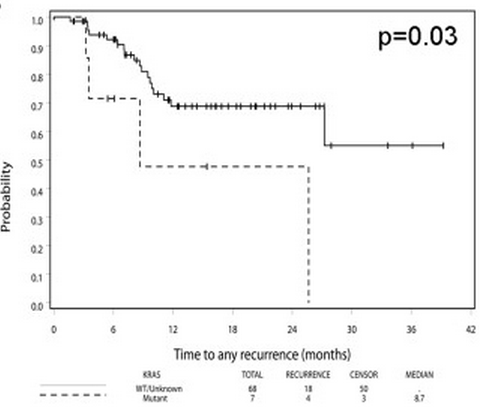
\includegraphics[width=\textwidth]{kaplanmeier.png}
  \caption{\textbf{Time to recurrence}}
  \label{kaplanrecurrence}
  \end{subfigure}
  \begin{subfigure}[b]{0.4\textwidth}
  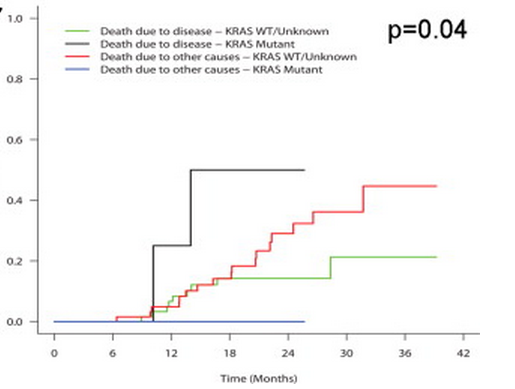
\includegraphics[width=\textwidth]{diseasedeath.png}
  \caption{\textbf{Death due to disease; K-Ras mutant, black}}
  \label{kplandeath}
  \end{subfigure}
  \caption{Kaplan-Meier plots of K-Ras mutant vs. wild-type prognosis \cite{mak2014}}
  \label{kraskaplan}
  \end{figure}
  

  \subsection*{Ras functional biophysics}
  The Ras family proteins are small GTPases; that is, they are enzymes which can bind GTP and hydrolyze it to GDP, which remains bound until an exchange \cite{pyla}. In its GTP-bound form, Ras is active, and engages downstream pro-growth signaling factors as seen in \Cref{growthfig}. Ras is then inactivated by hydrolyzing its bound GTP; however, this process is greatly assisted by a family of proteins known as GTPase Activating Proteins, or GAPs \cite{pyla}. 
    \begin{figure}[H]
  \centering
  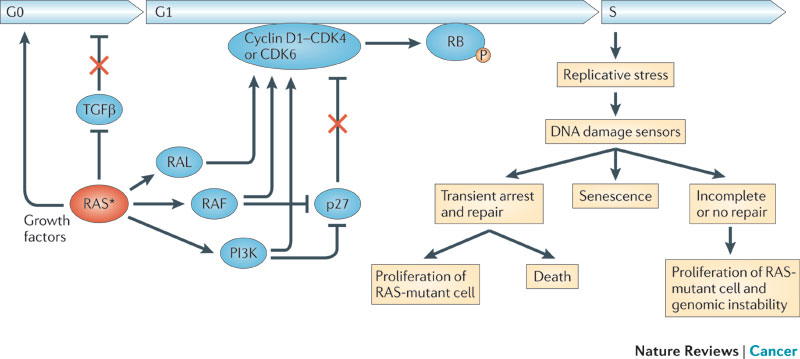
\includegraphics[width=0.5\textwidth]{ras_signal.jpg}
  \caption{\textbf{A diagram of major Ras growth signaling partners, indicating its connectedness in growth signaling pathways} \cite{pyla}}
  \label{growthfig}
  \end{figure}
  The oncogenic potential of K-Ras mutations relates to its central role in cellular growth signaling \cite{pyla}, as indicated by \Cref{growthfig}. This position in relevant pathways makes Ras both a critical means of cancer proliferation and an attractive drug target. However, its biophysical nature causes great difficulty in designing an inhibitor; first, oncogenic mutations generally ablate the ability for Ras to hydrolyze GTP, as well as its ability to interact with partners that assist in hydrolysis and thus become inactive \cite{pyla}. This loss-of-function mutation means that inhibition of the enzymatic activity is not a feasible avenue. Furthermore, outcompeting bound GTP is generally regarded as infeasible due to its picomolar affinity for GTP \cite{ostrem2013} , and the lack of any other apparent  binding sites in crystal structures \cite{ostrem2013}.
  
  \section*{Approach}
  \subsection*{Aim 1: Computationally map conformations accessible to Ras along with their corresponding energetics to identify potential opportunities for allosteric modulation}
  
  \subsubsection*{Hypothesis}
  Ras family proteins can adopt multiple kinetically metastable conformations, some of which are signaling-inactive and expose druggable binding sites for stabilizing ligands
  \subsubsection*{Overview:}
  As discussed above, Ras is a key protein in the ability for cancer cells to grow and divide, but the loss-of-function nature of its mutations and lack of apparent druggable sites render it a difficult target. While no apparent viable sites for ligand binding are present in crystal structures, there is evidence that there exist lower-populated conformations \cite{fesik} \cite{ostrem2013} which contain ligand binding sites, and may be signaling-inactive. Discovery of such sites allows us to rationally design ligands that can stabilize these inactive conformations, thus potentially inhibiting oncogenic growth signaling and leading to a new path to cancer therapeutics. In order to discover these conformations, we will use parallel high-throughput molecular dynamics to generate trajectory data, and Markov State Modeling (MSM) \cite{chodera2014} to combine the trajectory data into a conformational map, as conceptually illustrated in \Cref{craikfig}.
  
    \begin{figure}[H]
  \centering
  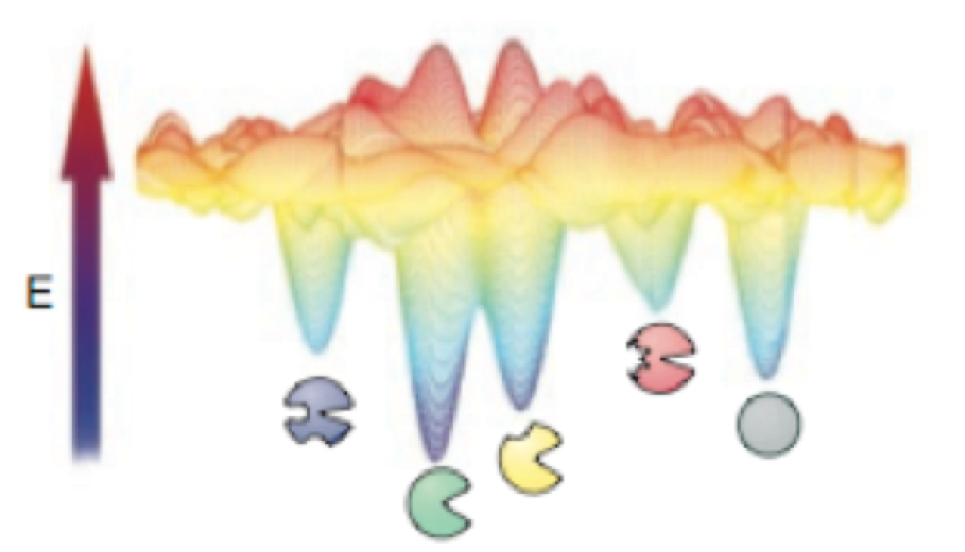
\includegraphics[width=0.5\textwidth]{craik.png}
  \caption{\textbf{A schematic of an energy landscape with multiple wells for metastable states} \cite{craik}}
  \label{craikfig}
  \end{figure}
  
  \subsubsection*{Objective 1: Identify metastable conformations and the associated energetics of oncogenic K-Ras using Markov State Model approaches}
  While there exists structural data as referenced elsewhere, little information exists regarding the dynamics of Ras proteins, despite their important role in cancer. Here we propose to use parallel molecular dynamics simulations with OpenMM \cref{openmm}, and to combine the independent trajectories using Markov State Model approaches \cref{chodera2014} to elucidate the conformational populations of oncogenic K-Ras and their kinetics. We also propose to use techniques developed in our laboratory to accelerate sampling, described below. The completion of this will give us unprecedented insight into opportunities for drugging this target.
  
 \underline{Markov State Modeling:} This process involves several steps. First, as the trajectory data is very high-dimensional, we will use a dimensionality-reduction technique, such as time-lagged independent component analysis (tICA) \cite{perez2013}. This technique transforms input coordinates, such as distances or torsions, into a new set of coordinates, highlighting the slowest degrees of freedom \cite{chodera2014}. Next, a technique such as Voronoi tessellation is used to assign the reduced-dimension trajectories to discrete states \cite{chodera2014}. These now-discretized trajectories are used to estimate the transition matrix between states \cite{chodera2014}. By using a maximally-connected subset of states in this final step, avoiding the inclusion of potentially problematic simulations of irrelevant conformational states \cite{kyle}. 
 
    \underline{Initialization with starting structures:} Despite the use of parallel, high-performance computing hardware, it remains difficult to fully sample the conformation space of a protein. In order to more rapidly and effectively sample the conformational states of K-Ras, we will use a pipeline developed in our laboratory that identifies protein structures in the protein data bank (PDB) by BLAST \cite{blast} sequence similarity, then constructs homology models of the target sequence using MODELLER \cite{modeller}, followed by a brief molecular dynamics refinement as shown in \Cref{msmseeder}. By starting from diverse conformations, we expect to more rapidly cover conformational space in the MD trajectories.
      
   \underline{Massively Parallel Molecular Dynamics (MD):} After generating the initial conformations, we will run explicit-solvent molecular dynamics on the starting structures, creating several copies of each with randomized starting velocities. This work will be performed primarily using Oak Ridge National Lab's Titan, the second-fastest civilian supercomputer in the world, for which we have been allocated compute time. We will use OpenMM \cite{openmm}, an open-source, high-performance molecular simulation package, to obtain trajectories for analysis. Initially, we will be simulating the G12C mutant, as it is both clinically relevant and the subject of recent investigation \cite{ostrem2013}, as well as the apo form of the K-Ras protein. We intend to repeat this protocol for GDP- and GTP- bound forms, as well as other clinically-relevant mutants.
  

  
  \begin{figure}[H]
    \centering
    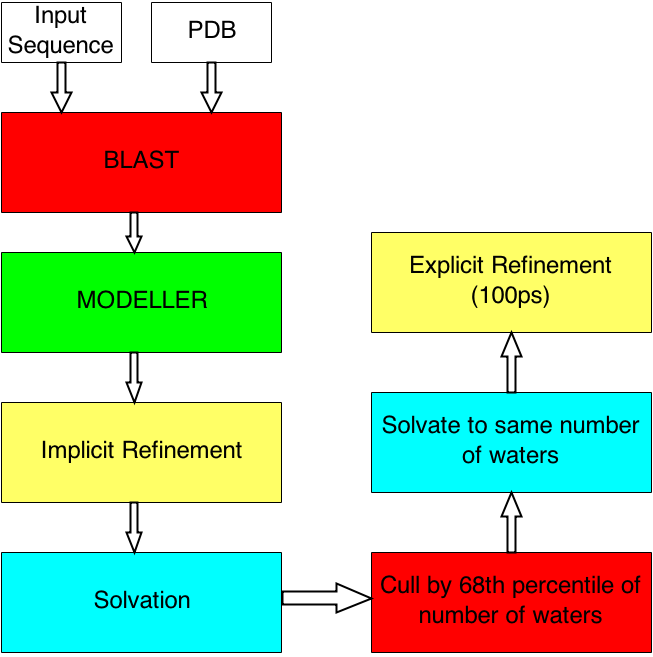
\includegraphics[width=0.5\textwidth]{msmseeder-diagram.png}
  \caption{\textbf{A flowchart demonstrating the generation of starting conformations.}}
  \label{msmseeder}
  \end{figure}
  

  
  \underline{Analyzing trajectory data:} As trajectory data is received from Titan, we will proceed by creating an MSM of the conformations of K-Ras.  
  
  \underline{Analyzing MSM Output:} The output of the MSM analysis will render several important pieces of information. First, it will enumerate a set of metastable conformations adopted by K-Ras. Moreover, the model will also yield the kinetics and energetics of these conformations, allowing us to identify near-ground state conformations in K-Ras.
  
  \subsubsection*{Objective 2: Mine the Metastable Conformations for potential ligand binding sites}
  The creation of a Markov State Model for Ras will provide us with unparalleled insight into this protein's conformational populations. With this data, we can begin searching for opportunities for allosteric modulation; to do so, we will look for conformations that contain potential ligand binding sites, as well as conformations which display similarity to the GDP-bound (inactive) conformation, especially in the Switch I and II effector regions displayed in \Cref{rasres}, as described below. We expect that this will lead to new avenues for therapeutic lead discovery.
  
  \underline{Elucidating excited state conformations:} Since our aim is to allosterically target Ras by stabilizing an inactive conformation with a small molecule, we will confine our search to metastable conformational states that are within 10$k_BT$ of the ground state. Conformations beyond this energy level would likely be difficult to stabilize with a small molecule \cite{kuntz1999}.
  
  \underline{Discovering Potential Small Molecule Binding Sites:} With this computational approach, we are afforded the opportunity to discover novel ligand binding sites that were not visible in experimental structures. We intend to screen the identified conformations with an algorithm known as LIGSITE \cite{hendlich1997}. This technique searches for points nearly-surrounded by solvent-inaccessible regions \cite{hendlich1997}. We believe that this will be successful for two reasons. First, this, approach has been used before to discover known cryptic binding sites in simulations without ligand \cite{bowman2012}, as illustrated in \Cref{bowmanbetalac}. 
  
  \begin{figure}[H]
  \centering
  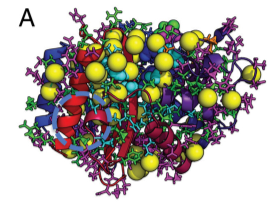
\includegraphics[width=0.5\textwidth]{betalac_cryptic.png}
  \caption{\textbf{An example of the identification of cryptic binding sites from MSM data on $\beta$-lactamase}. The known allosteric binding site is circled in blue, identified via MSM techniques without ligand. \cite{bowman2012}}
  \label{bowmanbetalac}
  \end{figure}
  Second, the existence of weakly-binding molecules to allosteric sites on K-Ras, such as the covalent inhibitors in \cite{ostrem2013} depicted in \Cref{shokat_mols}, whose bound structure is illustrated in \Cref{shokatfig}. In the case of the Shokat lab, this molecule was discovered by a screening technique that requires covalent attachment, and still relies on serendipity. Our approach can discover allosteric sites without first requiring an allosteric ligand, allowing for rational allosteric drug design. 
  \begin{figure}[H]
  \centering
  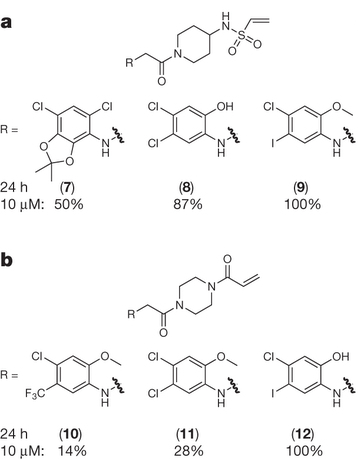
\includegraphics[width=0.4\textwidth]{shokat_mols.png}
  \caption{\textbf{Several molecules identified in \cite{ostrem2013} to inhibit K-Ras G12C.} Note the presence of an electrophile for covalent attachment to the required cysteine.}
  \label{shokat_mols}
  \end{figure}
  
  \begin{figure}[H]
  \centering
  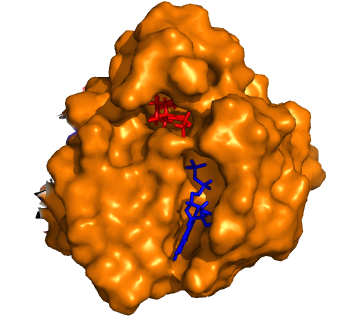
\includegraphics[width=0.5\textwidth]{4LV6.png}
  \caption{\textbf{K-Ras G12C with bound inhibitor, in red.}\cite{ostrem2013}. The presence of the inhibitor reveals an allosteric pocket above the nucleotide (blue) binding site in PDB entry 4LV6.}
  \label{shokatfig}
  \end{figure} 

  \subsubsection*{Objective 3: Identify putative druggable signaling-inactive conformations}
  Once we have identified metastable conformations, it is not only important to locate opportunities for ligand binding, but also to investigate which states may be less capable of transmitting a growth signal.
  
  \underline{Favoring the GDP-bound form: } The Shokat K-Ras inhibitor was shown to cause K-Ras to favor its GDP-bound form instead of its active GTP bound form.\cite{ostrem2013}. Thus, we will search for conformations which are more similar to the GDP bound conformations such as those found in PDB codes 4LPK and 4LRW using metrics such as RMSD, as well as placement of key residues involved in nucleotide binding.
  
  \underline{Disrupting interaction with Raf or PI3K:} Key interaction partners of Ras family proteins include SOS, an upstream effector that encourages nucleotide exchange, Raf, a group of protein kinases, and PI3K \cite{pyla}. Comparison of available crystal structures of Ras-family proteins bound to these effectors with structures of inactive Ras can also lend insight into which conformational features are required for Ras activity \cite{pi3k}, such as those indicated in \Cref{raspi3kinteraction}. 
  \begin{figure}[H]
  \centering
  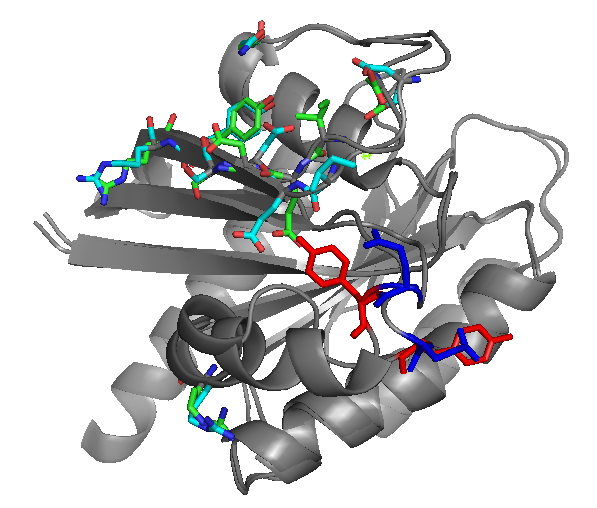
\includegraphics[width=0.5\textwidth]{ras_actvinact.png}
  \caption{\textbf{Alignment of GDP and GTP bound conformations of H-Ras, showing positioning of PI3K-interacting residues \cite{pi3k}.} PDB codes: inactive 1Q21 \cite{rasgdp}, green side chains, active 5P21\cite{rasgtp}, teal side chains. Red and blue side chains denote dramatically different positioning between active and inactive forms, respectively.}
  \label{raspi3kinteraction}
  \end{figure}
  
  \subsubsection*{Objective 4: Experimentally validate predicted conformational populations}
  
  Once we have constructed a computationally useful MSM of Ras, it is important to perform experiments to validate that we have actually modeled the system in a relevant manner. To that end, I will develop several techniques to biophysically examine the perturbation of conformational populations of Ras.

\underline{Free energy calculations with known ligands:} We will perform free energy calculations on known Ras ligands, such as those in \cite{fesik} , weighting each free energy by the predicted probability of adopting that conformation. If the conformational populations are predicted correctly, the free energy calculations should give a similar value to measured binding affinity.
  
\underline{Fluorescent labeling of Ras:} We will also use an assay involving the introduction of multiple minimally-perturbative tryptophan mutants as described in \cite{trpmut}. Depending on their location, these mutants can be used to confirm binding of a ligand (if the tryptophan is near the binding site) or a conformational change upon ligand binding (if the tryptophan is distant from the binding site). We intend to use known ligands to perturb tryptophan-mutant Ras, and compare fluorescence results to the predicted conformational populations in the MSM.

  \subsubsection*{Anticipated Results}
  We anticipate that this aim will generate a valuable model of the conformational landscape of K-Ras, including potentially inactive conformations that expose putative ligand binding sites. We have high confidence that this will be possible, as there are several allosteric ligands known already \cite{ostrem2013} \cite{fesik}, albeit with serious shortcomings---those that bind tightly enough to be useful are covalent inhibitors, and therefore require the presence of a cysteine at the binding site. Where our method provides considerable improvements over currently available data and techniques is in creating a map of the conformations of K-Ras, with associated kinetics and energetics---these are quantities that are difficult, if not impossible, to determine from bound structures of serendipitously discovered allosteric modulators.
  
  \subsubsection*{Potential Problems and Alternative Approaches}
  
  \underline{The forcefield may be inaccurate:} It is conceivable that the classical forcefields used in molecular dynamics are either incorrectly parameterized or insufficiently detailed to recapitulate conformational populations. To that end, our laboratory is engaged in collaborative projects to benchmark and improve forcefields and their parameters. However, recent studies of forcefields show continuing improvement, as indicated in \Cref{forcefig}, where lower scores are better \cite{deshaw} and suggest that the problem may not be so dire. 
  \begin{figure}[H]
  \centering
  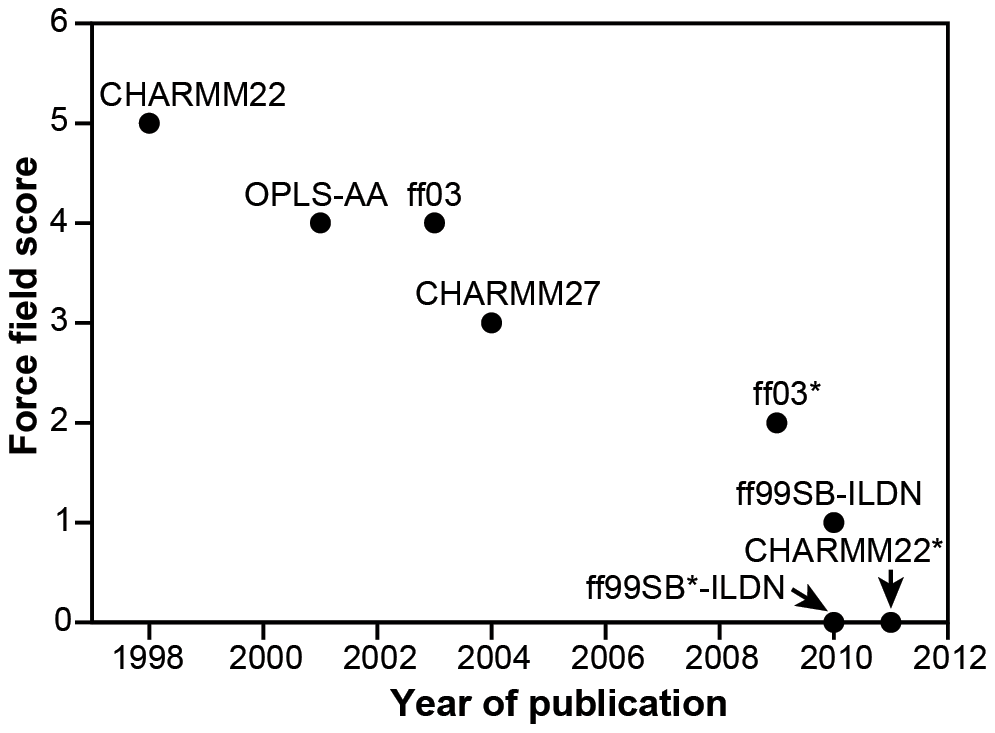
\includegraphics[width=0.5\textwidth]{foldingmark.png}
  \caption{\textbf{A comparison of forcefields over time}\cite{deshaw}. Lower scores indicate better agreement with experiment, demonstrating consistent improvement.}
  \label{forcefig}
  \end{figure}
  
  
 \underline{There may be no identified conformations with binding pockets:} This seems highly unlikely, given the existence of demonstrated binding pockets \cite{ostrem2013} \cite{fesik}, but in this event we can screen against the binding pockets identified in  \cite{ostrem2013} and \cite{fesik}.
  
 \underline{Minimally-perturbative tryptophan mutants may not be possible at the required sites:} As an alternative to labeling via tryptophan mutants, we can use fluorescent labeling on surface cysteines in the region of interest to probe conformational populations.
  
  \underline{Compare MSM conformational population to NMR results:} If the above methods prove inconclusive, we intend to compare the conformational populations obtained via MSM to NMR data such as NOE.
  
  
  
  
\subsection*{Aim 2: Identify new small molecule ligands of Ras}
\subsubsection*{Hypothesis}
Virtual screening can identify fragment-like compounds that bind to putative allosteric sites from Aim 1.

\subsubsection*{Objective 1: Perform virtual screening on a library of commercially-available compounds against putative allosteric binding sites}

Once we have identified suitable metastable conformations, we intend to begin a virtual screen with a large library of purchasable drug-like fragments. This will allow us to discover new scaffolds for allosteric Ras ligands, and is an important step in the direction of novel Ras inhibitor design.

\underline{Retrieve database of readily available fragment-like compounds:} Databases such as ZINC \cite{irwin2012} can provide collections of molecules that are readily available for purchase and meet certain criteria. We intend to begin by virtual screening compounds in the "Frags now"  database, which is a database of over 1 million readily-available "fragment-like" (predicted logP$\leq$3.5, molecular weight$\leq$250, and the number of rotatable bonds$\leq$5). We will also filter by solubility, as the initial assays will take place at high concentration. The choice of the fragment database will allow us to screen a broad area of drug-like chemical space.

\underline{Use small molecule docking to discover potential hits against relevant conformations:} Once potentially inactive conformations have been identified, we intend to perform a docking-based virtual screen of our library agains these conformations, targeted at the potential binding sites for a small molecule. We will use a variety of docking tools to perform this screen after testing for known ligand binding over decoys. Molecular docking is a technique that uses a scoring function based on select features of the protein and ligand. While it often omits important features of the interaction, docking can be used to enrich a large library of compounds for potential hits. \cite{dockingrev}

\subsubsection*{Objective 2: Filter hits using alchemical free energy calculations:}

\underline{Highest scoring compounds are enriched for binders:} Although docking makes many approximations, it has been shown that docking with a large library of molecules leads to an enrichment among the highest-scoring molecules for potential hits. Therefore, we will use the top 1\% of the screening results, filtered by physical properties such as solubility, for this stage.

\underline{Free energy calculations:} Because docking is not typically able to produce an accurate binding affinity\cite{warren2006} we will use the more rigorous alchemical free energy calculations on the enriched set from docking. These methods create multiple systems which are "alchemically" modified; that is, the ligand and protein are decoupled to varying degrees, from completely interacting to completely non-interacting. Free energy differences, along with error estimates, are then calculated between each state\cite{boresch2013}.

\subsubsection*{Objective 3: Experimentally measure binding affinities of hits}

\underline{Test differential affinity for GDP and GTP:} If the identified putative inhibition of Ras involves the stabilization of a GDP-favored conformation as in \cite{ostrem2013}, we intend to test the compound's ability to bias Ras toward a GDP-bound form. We will follow the protocol outlined by Ostrem, et al. \cite{ostrem2013}. This assay begins with mant-GDP-loaded Ras, which is fluorescent. The assay then titrates in unlabeled GTP, or a nonhydrolyzable analog, and measures the change in fluorescence as a result. As shown in \Cref{gtpassay}, if the ligand actually biases Ras toward a GDP-bound conformation, a shift from untreated Ras should be seen, denoting a decrease in affinity for GTP. As a control, both ligand-bound and ligand-free Ras should be titrated with unlabeled GDP, and there should be no difference in the change in fluorescence vs. concentration GDP. 

\begin{figure}
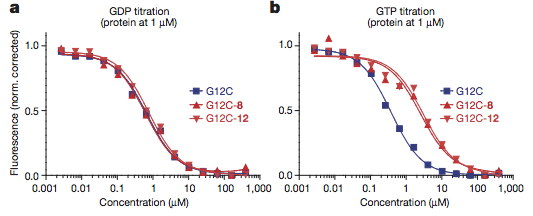
\includegraphics[width=\textwidth]{shokatassay.png}
\caption{\textbf{As demonstrated here, perturbation with a hit should result in a shift in the affinity for GTP} \cite{ostrem2013}}
\label{gtpassay}
\end{figure}

\underline{Test modulation of conformational populations with fluorescent labeling:} We will use the assay developed in Aim 1, validated on known Ras ligands, to experimentally test the fragments discovered in our virtual screen.

\subsubsection*{Anticipated Results}

Out of the large library of over 1,000,000 fragment-like molecules in the "frags now" database of ZINC \cite{irwin2012}, we expect docking to enrich a collection of molecules for fragments that will more likely bind to the predicted binding cavity. We further expect that that binding to sites exposed only in excited state conformations will perturb the equilibrium conformational populations of Ras in a ligand concentration-dependent manner detectable by our fluorescence assay. Finally, we expect that the results of this stage will be useful leads to pursue tighter-binding derivatives and a set of much-needed starting points for allosteric Ras modulators.

\subsubsection*{Potential Problems and Alternative Approaches}

While we expect the large library of available fragments to contain some hits, there are potential issues

\underline{The fragment database may not contain any binding ligands:} It is possible that the database we will use does not contain any binding ligands, or contains only ligands that bind so weakly that the effect is undetectable even at the solubility limit. This might be evidenced by few high-scoring docking poses, or free energy calculations that suggest no binding. To resolve such an issue, we would seek other screening libraries, such as a library used internally at Memorial Sloan Kettering, or other libraries on ZINC.

\underline{Docking may not accurately score ligands:} This problem would be evidenced by free energy calculations showing no significant improvement of binding affinity among high-scoring docking results \cite{warren2006}, or a failure to distinguish known ligands from decoys. This is a significant issue \cite{warren2006}, which we would first attempt to resolve by adding various amounts of detail to the docking calculations. Absent improvement, we could potentially turn to previously-discovered scaffolds such as those by Fesik, et al. \cite{fesik} or Ostrem, et al.  \cite{ostrem2013}.


\subsection*{Aim 3: Computationally explore chemical space near identified ligands}
Often, when hits are discovered, medicinal chemists use their chemical intuition and available chemistry to explore chemical space near the hit. However, this can be error-prone, time-consuming, and costly, especially as one realizes the combinatorial explosion of possible modifications of only a single hit. We propose instead to use a rigorous statistical mechanics framework to computationally explore the chemical space near derivatives of the scaffold to improve binding affinity. Using the theory of expanded ensemble simulation\cite{lyubartsev1992}, we will allow the lead to change various chemical substituents during simulation, biased toward tighter-binding ligands. 


\subsubsection*{Hypothesis}
Expanded-ensemble techniques that allow simulations to explore chemical space can identify novel chemical motifs necessary for binding to a specific protein.

\subsubsection*{Objective 1: Perform expanded-ensemble simulations on synthetically-feasible derivatives of the identified leads}

\underline{Synthetic feasibility model:} We intend to use a database of chemical transformations, curated by medicinal chemists, to identify potential transformations of our ligand. These databases, such as \cite{chemtransform}, can allow us to make proposed transformations, such as the transformation indicated in \Cref{transfig}.

\begin{figure}[H]
\centering
 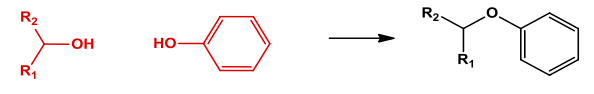
\includegraphics[width=0.7\textwidth]{chem_trans.png}
 \caption{\textbf{An example of a chemical transformation that can be used in simulation} \cite{chemtransform}}
 \label{transfig}
 \end{figure}


\underline{Chemical space becomes combinatorially large:} As indicated in \Cref{markfig}, even a scaffold with four potential sites for modification and 10 modifications at each site can result in a search space of $10^4$ molecules. This is difficult both for traditional medicinal chemistry and for free energy calculations. Therefore, to computationally explore this combinatorially large chemical space, we propose to use expanded ensemble simulation \cite{lyubartsev1992}, as described below. 
\begin{figure}[H]
\centering
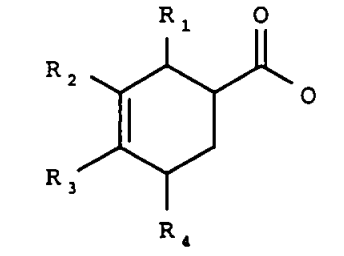
\includegraphics[scale=0.4]{mark.png}
\caption{\textbf{An example of a Markush structure, containing combinatorially many possibilities} \cite{mark}}
\label{markfig}
\end{figure}
\underline{Expanded ensemble simulation:} While simulation of biomolecules and ligands often proceeds via sampling (molecular dynamics or Markov Chain Monte Carlo) from the canonical ensemble, whose equilibrium distribution is given by \begin{equation} \pi(\textbf{x})=\frac{\exp[-u(\textbf{x})]}{\int \exp[-u(\textbf{x})] \mathrm{d}\textbf{x}}=Z^{-1}\exp[-u(\textbf{x})]\end{equation}
where \textit{u}(\textbf{x}) represents the reduced potential, given in its general form by

\begin{equation} \label{reducedu} u(\textbf{x})=\beta[U(\textbf{x})+pV(\textbf{x})+\boldsymbol\mu^T\textbf{n}(\textbf{x})] \end{equation}
where \textbf{x} is the configuration of the system, U(\textbf{x}) is the potential energy, V(\textbf{x}) is the volume (for a constant pressure simulation), p is the external pressure, and $\boldsymbol\mu$ is the chemical potential of each particle represented in \textbf{n}(\textbf{x}), which represents the number of particles in a (semi) grand canonical simulation \cite{shirts2008}. $Z$ represents the partition function, that is, the integral of $\exp[-u(\textbf{x}))$ over its entire domain. However, we need not restrict ourselves to this; we can define an \emph{expanded ensemble} such that we instead sample from a joint distribution given by \begin{equation} \label{eq:exens} \pi(\textbf{x},k)=\frac{\exp[-u_k(\textbf{x})+g_k]}{\sum_{i=1}^{k}\int \exp[-u_i(\textbf{x})+g_i] \mathrm{d}\textbf{x}} \end{equation} where the new parameter \textit{k} indexes the state of the simulation, and its corresponding $u_k$ gives the the reduced potential for that state and configuration. In our case, the state $k$ represents the current molecule, and a jump to a different state would represent a jump to a different ligand molecule. We also have the free parameter $g_k$, which enables us to weight each state with a biasing potential. Sampling from \Cref{eq:exens} often proceeds by Gibbs sampling \cite{liu}; that is, we draw a correlated sample from the conditional of \textbf{x} given \textit{k},
%
\begin{equation} \label{eq:xgivenk} \pi(\textbf{x}|k)=\frac{\exp[-u_k(\textbf{x})]}{\int \exp[-u_k(\textbf{x})] \mathrm{d}\textbf{x}} \end{equation}
%
followed by a sample from the conditional of \textit{k} given \textbf{x}:
%
\begin{equation} \label{eq:kgivenx} \pi(k|\textbf{x})=\frac{\exp[-u_k(\textbf{x})+g_k]}{\sum_{i=1}^{k}\exp[-u_i(\textbf{x})+g_i]} \end{equation}
%
\underline{Biasing the simulation toward tighter binders:} We will show that, for a specific convenient choice of the weights $g_k$, the marginal distribution $\pi(k)$ is proportional to the binding affinity, $K_a$, such that the expanded ensemble simulation will be driven to spend more time in chemical states that are tighter binders.  This will enable expanded ensemble simulations to effectively hunt through large chemical spaces for good ligands. In order to derive this, we first marginalize out \textbf{x} in \Cref{eq:kgivenx}:
\begin{equation} \label{eq:marginalk} \pi(k)=\frac{\exp(g_k)\int \exp[-u_k(\textbf{x})] \mathrm{d}\textbf{x}}{\sum_{i=1}^{k}\int \exp[-u_i(\textbf{x})+g_i] \mathrm{d}\textbf{x}}\propto\exp(g_k)Z_{PL_k}} \end{equation}

where $Z_{PL_k}$ represents the partition function for the protein-ligand complex \textit{k}.
We also know from thermodynamics that binding affinity, excluding multiplicative constants, is calculated as \cite{gilson1997}
\begin{equation} \label{eq:binding}K_a \equiv \frac{[PL]}{[P][L]} \propto \frac{Z_{PL}}{Z_{P\emptyset}} / \frac{Z_L}{Z_\emptyset} \end{equation}
%
and since the partition functions of the solvent alone and protein alone will not change during our expanded ensemble calculations, \Cref{eq:binding} is proportional to
%
\begin{equation} \label{eq:propbind} \frac{Z_{PL}}{Z_{L}} \end{equation}
%
Thus, setting the weight $g_k=-ln(Z_{ligand_k})$ yields an unnormalized probability for being in state \textit{k} of
%
\begin{equation} \label{eq:biasedk} \pi(k) \propto \frac{Z_{PL_k}}{Z_{L_k}} \end{equation}
%
which is equivalent to the expression in \Cref{eq:propbind}. Therefore, by using a specific $g_k = -lnZ_{L_k}$, which we can approximate with  the hydration free energy in explicit or implicit solvent (discussed below), we can steer the simulation toward molecules with better $K_{a}$ naturally.


\underline{ Use Nonequilibrium Candidate Monte Carlo (NCMC) moves for explicit-solvent simulation:} Though the above framework is theoretically sound, the presence of explicit waters near the site of transformation may create very low acceptance rates for state-change proposals, as there will likely be a clash if the ligand is instantaneously modified. We intend to take advantage of recent work \cite{nilmeier2011} that has shown that one can make nonequilibrium moves and preserve the equilibrium distribution. Using this scheme, we would not simply propose to instantaneously change the state, but rather propose a protocol to transition between the current state and the next proposed state, interleaving partial perturbation steps with propagation steps. The final move is then accepted or rejected based on the nonequilibrium work performed, and, to preserve the equilibrium distribution, momenta are reversed if the move is rejected. As shown in \Cref{ncmcfig}, for the test case of a WCA dimer, the use of NCMC dramatically increased acceptance rates and dramatically decreased correlation times.

\begin{figure}
\centering
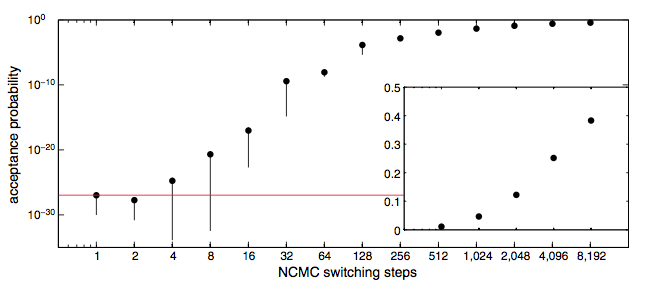
\includegraphics[width=0.6\textwidth]{ncmc.png}
\caption{\textbf{NCMC can improve the acceptance rates of MC moves (such as those that will be used to propose changes in chemical identities) by orders of magnitude.}\cite{nilmeier2011}}
\label{ncmcfig}
\end{figure}


\subsubsection*{Objective 2: Test whether single point energies of minimized ligands are sufficient to bias the simulation toward tight binders }


\underline{Setting bias to a single point energy is a useful approximation to unbound partition function:} Although the above is tantalizing, calculating the normalizing constant of the ligand (equivalent to its hydration free energy) is nontrivial. Therefore, we propose to use single point energies, given by a simple evaluation of the forcefield at a minimized conformation in implicit solvent to provide an estimate for the weight to use in expanded ensemble simulation. This choice is motivated by recent work \cite{mobley2008} indicating that though point energies of ligands may be insufficient for calculating hydration free energy estimates, they are relatively close (RMSE=0.39$\pm$0.05 kcal/mol for minimized ligands in solvent) \cite{mobley2008}. Because the single point estimates are relatively close to the hydration free energy values, we would expect them to still bias our expanded ensemble in the correct direction to discover tighter-binding ligands. 


\subsection*{Objective 3: Test whether compounds identified via the expanded-ensemble method will bind more tightly to oncogenic K-Ras and potentially disrupt its phenotype}

Once we have obtained simulation statistics in the expanded-ensemble technique described above, we will move to confirm that these ligands actually bind to oncogenic K-Ras.

\underline{Perform free energy calculations on derivatives:} The first step in confirming that these ligands bind is to run alchemical free energy calculations on the top-scorers, confirming that they bind to a considerable enough degree to warrant synthesis and wet lab experimentation. This is done because free energies of binding can be computed much more precisely this way than looking at $-kT ln \pi(k)$ from the expanded ensemble simulation.

\underline{Collaborate with organic synthesis core to have derivatives synthesized:} Since we have started with purchasable fragments and derivatized them \textit{in silico}, we will collaborate with the organic synthesis core at Memorial Sloan Kettering to have the derivatives synthesized for \textit{in vitro} testing.

\underline{Biophysical assay for GDP preference:} If the conformation being stabilized is one that we predict to prefer GDP (for instance, by similarity to the GDP-bound conformation), we will use the GTP-GDP preference assay described above to compare the affinity of our optimized ligand to the original fragment.

\underline{Fluorescently labeling positions on the protein:} We will also use fluorescence assays developed in Aim2 to compare the ability of the optimized ligands to affect the conformational populations of Ras with the corresponding unoptimized fragments.

\underline{Perform Isothermal Titration Calorimetry:} This technique, very popular and important in binding affinity measurement \cite{itcref} measures the heat released by ligand binding by monitoring the amount of heat required to keep a reference cell at the same temperature as a sample cell, into which ligand is titrated. ITC has been used for fragment-based studies \cite{drinkwater2010}, indicating that it is viable even for compounds with weak affinity. Additionally, our lab is developing new techniques to cope with low-affinity ITC. This technique is useful for measuring whether the ligand binds at all, and with what affinity. Due to the large amount of ligand required, however, its use may be limited for low-solubility compounds.
s
\underline{Assay the effect of the ligand on cell growth:} We will collaborate with cancer biologists to assay the ligand in inhibiting cancer cell growth, in both cells dependent on Ras and cells with Ras knocked out to control for 
nonspecific binding, following a protocol similar to that followed by Ostrem, et al. \cite{ostrem2013}.

\underline{Engage structural biology collaborator for structural evidence of binding:} After demonstrating that the ligand successfully binds and has an effect on cancer growth, we will contact a structural biology collaborator at Stony Brook University to assist us in generating X-ray crystal or NMR evidence of the bound pose of the ligand and K-Ras.

\subsubsection*{Anticipated Results}

\underline{Expanded ensemble simulation techniques will improve ligand affinity:} We expect that subjecting our lead compounds identified in the previous screen to our technique of expanded-ensemble simulation will identify derivatives that are both synthetically realistic and tighter binders. We anticipate that this result will also indicate novel chemical motifs that may be relevant in targeting Ras, and may suggest a general approach for identifying relevant chemical space for targeting a particular protein/binding pocket. We furthermore expect that the ligand will stabilize the expected conformation and cause measurable changes in the activity of Ras. This will help pave the way for the development of novel anticancer drugs targeting this heretofore very difficult-to-target protein.

\subsubsection*{Potential Problems and Alternative Approaches:}

\underline{The synthetic feasibility model may need refinement:} Synthetic feasibility models curated by medicinal chemists may not always reflect what is synthetically feasible on every scaffold that matches the pattern. As an alternative, if we are generating very unrealistic proposals, we can limit the scope of the modifications, as well as restrict the modifications available to a particular lead based on curation in greater detail.

\underline{The single point-energy estimate may be a poor approximation for complex ligands:} For ligands with high entropic contributions, the point-energy estimate may prove insufficient. As a replacement, the more computationally costly but more rigorous approach of using solvation free energies can be substituted.

\underline{The large number of weakly-binding derivatives can overwhelm the small number of tight binders:} It is possible that the very large number of weakly-binding variants that can be visited in a simulation will overwhelm the small number of tightly-binding derivatives. To combat this issue, we will explore techniques to amplify the bias toward very tightly-binding ligands.

\underline{Fluorescence-based methods may not reveal relevant activity even if it exists:} If the predicted conformational or nucleotide-preference changes do not occur, the fluorescence measurements may report no change. To combat this and confirm the negative, we will use techniques such as isothermal titration calorimetry (ITC), which are label-free and can confirm that no binding within detection limits is occurring. 

\section*{Conclusion}
Once completed, our technique will have accomplished several innovations. First, we will have produced novel ligands that target and stabilize Ras family proteins, providing a new avenue for development of therapeutics targeting this "undruggable" target. We will also have produced a map of the conformational populations of Ras, enabling further studies of its functional biophysics, critical to understanding the oncogenic potential of Ras. Furthermore, as our technique is a systematic one, it will serve as a template for the discovery of allosteric sites and ligands, as well as a rigorous technique for the improvement of scaffold binding in the face of combinatorially-large chemical space.

\clearpage

\bibliographystyle{unsrt}  
\bibliography{\jobname}  




\end{document}

